\documentclass[xcolor=table]{beamer}

\useinnertheme{metropolis}
\useoutertheme{metropolis}
\usecolortheme{metropolis}
\usefonttheme{professionalfonts}         % Use metropolis theme

\usepackage{fontspec}
\setsansfont{Fira Sans Light}
\setmonofont{Fira Mono}
\setmainfont{Fira Sans Light}

\usepackage[bibstyle=unified, citestyle=unified, backend=biber]{biblatex}
\addbibresource{fdsl.bib}

\usepackage{longtable}
\usepackage{tipa}
\usepackage{booktabs}
\usepackage{tikz}
\usepackage{tikz-qtree}
\usepackage{expex}
\usepackage[normalem]{ulem}
\usepackage{xcolor}
\usepackage{float}
\usepackage{etoolbox}
\usepackage{multirow}
\usepackage{graphicx}
\usepackage{wrapfig}
\usepackage{subfig}
\usepackage{mathabx}
\usepackage{hyperref}

\usetikzlibrary{matrix}
\usetikzlibrary{positioning}
\usetikzlibrary{arrows.meta}
\usetikzlibrary{tikzmark}
\usetikzlibrary{decorations.shapes}

\tikzset{mytree/.style={baseline=(top.base),
level distance=2.5em, sibling distance=4em, align=center,
parent anchor=south, child anchor=south, anchor=north}}

	\hypersetup{
		colorlinks=true,
		linkcolor=black,
		citecolor=magenta,
		filecolor=black,
    		urlcolor=black,
	}

\lingset{numoffset=1ex, belowglpreambleskip=0ex, aboveglftskip=0ex, belowexskip=2ex, aboveexskip=2ex} % gloss formatting


\renewcommand*{\bibfont}{\small}
\setbeamertemplate{bibliography item}{}


\AtBeginSection[]{
  \begin{frame}
  \vfill
  \centering
  \usebeamerfont{title}\insertsectionhead\par%
  \vfill
  \end{frame}
}


\title{Accounting for Russian superlatives with Nanosyntax}
\date{FDSL 15, 05.10.2022}
\author{Daniar Kasenov, NRU HSE / MSU\\ antidanyar@protonmail.com}

\begin{document}

	\maketitle
		
	\section{Introduction}

	\begin{frame}{Intro}

		\begin{itemize}

			\item This talk provides a Nanosyntactic analysis for Russian adjective degree morphology, following previous Nanosyntactic work (\cite{Caha:2019}; \cite{Caha:2020}; \cite{Caha:2022})

			\item Slides and general info available at github.com/antidanyar/

			\item Work supported by RSF grant \# 22-18-00285

		\end{itemize}

	\end{frame}

	\begin{frame}{Basic adjectival morphology in Russian}

		Take \textit{krasiv-yj} `beautiful'

		\textit{krasiv-ee} `more beautiful' / \textit{bolee krasiv-yj}

		\textit{krasiv-ej-sh-yj} `the most beautiful' / \textit{nai-krasiv-ej-sh-yj} / \textit{samyj krasiv-yj}

	\end{frame}

	\begin{frame}{Basic adjectival morphology in Russian}

		Take \textit{khorosh-yj} `good'

		\textit{luchsh-e} `better' / ?\textit{bolee khorosh-yj}

		\textit{luchsh-yj} `the most beautiful' / \textit{nai-luchsh-yj} / ?\textit{samyj khorosh-yj}

	\end{frame}

	\begin{frame}{Superlatives: combining strategies}

		\textit{samyj krasiv-yj} / \textit{*samyj krasiv-ej-sh-yj} / \textit{*samyj nai-krasiv-ej-sh-yj}

		Russian 1: *\textit{samyj khorosh-yj} / \textit{samyj luchsh-yj} / *\textit{samyj nai-luchsh-yj}

		Russian 2: \textit{samyj khorosh-yj} / *\textit{samyj luchsh-yj} / *\textit{samyj nai-luchsh-yj}

		I am strictrly a Russian 1 speaker $\Rightarrow$ talk is based on judgements of people who agree with Russian 1 judgement

	\end{frame}

	\begin{frame}{Puzzle one}

		\textit{samyj} is out with all other superlatives in regular adjectives, but is ok with bare suppletive superlatives for some speakers and isn't for others -- why?

	\end{frame}

	\begin{frame}{Puzzle two}

		Despite there being variation wrt. \textit{samyj khoroshyj/luchshyj} there is \textbf{none} wrt. \textit{nai-luchshyj}

		\textit{nai-khoroshyj} is always out -- why?
	\end{frame}

	\begin{frame}{Puzzle three}

		Take another two adjectives: \textit{plokh-oj} `bad', \textit{strog-ij} `strict', and compare that with \textit{krasiv-yj}

		\textit{plokh-oj} -- \textit{khuzh-e} -- \textit{khud-sh-yj}

		\textit{strog-ij} -- \textit{strozh-e} -- \textit{strozh-aj-sh-yj}

		\textit{krasiv-yj} -- \textit{krasiv-ej-e} -- \textit{krasiv-ej-sh-yj}

		What's up with \textit{strogij}?		

	\end{frame}

	\begin{frame}{Our goal}

		Main claim: all three puzzles are captured straightforwardly in a Nanosyntactic analysis of Russian degree morphology

		Assumptions: Nanosyntactic model of grammar (\cite{Starke:2010}); prefix theory of \textcite{Starke:2018}; degree structure of \textcite{Bobaljik:2012} and \textcite{Caha:2022}

	\end{frame}

	\section{Theoretical background}

	\begin{frame}{Comparative-superlative containment}

		\cite{Bobaljik:2012}: a study of suppletion in comparatives/superlatives

		Not attested: same root in positive/superlative, different root in comparative (*ABA)

		Based on *ABA, he proposed this structure: [SPRL [CMPR [ADJ]]]

	\end{frame}

	\begin{frame}{Spliiting CMPR}

	Czech: two types of comparative forms, with one affix clearly being contained in the other

	\textit{červen-ý} /  \textit{červen-ěj-š-í} `red'

	\textit{bohat-ý} / \textit{bohat-š-í} `rich'

	A straightforward solution: two COMP heads, one spells out as \textit{-ěj-}, other as \textit{-š-}

	\end{frame}

	\begin{frame}{Spliiting SPRL}

	Latin: two types of superlative forms, with one affix clearly being contained in the other

	\textit{alt-us} \textit{alt-i-or} \textit{alt-i-ss-im-us}
	
	\textit{mal-us} \textit{pe-i-or} \textit{pe-ss-im-us}

	\textit{bon-us} \textit{mel-i-or} \textit{opt-im-us}

	A straightforward solution: two SPRL heads, one spells out as \textit{-ss-}, other as \textit{-im-}

	\end{frame}

	\begin{frame}{Our structure}

		\begin{tikzpicture}[mytree, inv/.style={overlay, coordinate}, sibling distance=4em, level distance=1em]
					\node(top) {S2P}
					child {node {S2}}
					child {node {S1P}
						child {node {S1}}
						child {node {C2P}
							child {node {C2}}
							child {node {C1P}
								child {node {C1}}
								child {node {QP}
									child {node {Q}}
									child {node {aP}
										child{node {a}}
										child {node { {$\sqrt{\mbox{ROOT}}$ } }}
									}
								}
							}
						}
					}
					;
			\end{tikzpicture}

		Our goal: provide L-trees given this structure. Our puzzles, however, come from prefixal morphology. How does it work in Nanosyntax?

	\end{frame}

	\begin{frame}{Background: prefixes in Nanosyntax}

		Assume we have a tense-aspect-verb structure (example from Starke 2018)

		Suffix structure (born by movement of VP from Comp,AspP to Spec,TP):

		
		\begin{tikzpicture}[mytree, inv/.style={overlay, coordinate}, sibling distance=4em, level distance=1em]
					\coordinate(top)
						child {node {VP}}
						child {coordinate
							child {node {T}}
							child {coordinate
								child {node {Asp}}}}
					;
			\end{tikzpicture}

	\end{frame}

	\begin{frame}{Background: prefixes in Nanosyntax}

		Assume we have a tense-aspect-verb structure (example from Starke 2018)

		Prefix structure (built by parallel derivation that merges T and Asp independently):

		\begin{tikzpicture}[mytree, inv/.style={overlay, coordinate}, sibling distance=4em, level distance=1em]
					\coordinate(top)
						child {coordinate
							child {node {T}}
							child {node {Asp}}
						}
						child {node {VP}};
			\end{tikzpicture}

	\end{frame}

	\begin{frame}{Comparatives}

	Suffix: \begin{tikzpicture}[mytree, inv/.style={overlay, coordinate}, sibling distance=4em, level distance=1em]
					\coordinate(top)
						child {node {QP}}
						child {coordinate
							child {node {C2}}
							child {coordinate
								child {node {C1}}}}
					;
			\end{tikzpicture}
	Prefix: \begin{tikzpicture}[mytree, inv/.style={overlay, coordinate}, sibling distance=4em, level distance=1em]
					\coordinate(top)
						child {coordinate
							child {node {C2}}
							child {node {C1}}
						}
						child {node {QP}};
			\end{tikzpicture}

	Note: we should carefully track that Merge-F (suffix) is to be preferred to Merge-XP (prefix)

	Another note: we assume that there must be one-feature-overlap in merged XP and the main functional structure

	\end{frame}

	\section{Analysis}
	

	\begin{frame}{Puzzle one}

			\textit{samyj} is out with all other superlatives in regular adjectives, but is ok with bare suppletive superlatives	

			\begin{minipage}[t]{.3\textwidth}
			L-tree for \textit{samyj}\\
			\begin{tikzpicture}[mytree, inv/.style={overlay, coordinate}, sibling distance=2em, level distance=1.5em]
					\coordinate(top)
						child {node {S2}}
						child {coordinate
							child {node {S1}}
							child {coordinate
								child {node {S1}}  
								child {coordinate
									child {node {C2}}
									child {coordinate
										child {node {C1}}
										child {node {Q}}
									}
								}
							}}
					;
			\end{tikzpicture}
			\end{minipage}
			\begin{minipage}[t]{.3\textwidth}
			L-tree for \textit{luchsh-}\\
			\begin{tikzpicture}[mytree, inv/.style={overlay, coordinate}, sibling distance=2em, level distance=1.5em]
					\coordinate(top)
						child {node {C2}}
						child {coordinate
						child {node {C1}}
							child {coordinate
								child {node {Q}}
								child {coordinate 
									child {node {...}}
									child {node { $\sqrt{\mbox{good}}$ }}
								}
							}
						}
					;
			\end{tikzpicture}
			\end{minipage}
			\begin{minipage}[t]{.3\textwidth}
			L-tree for \textit{khorosh-}\\
			\begin{tikzpicture}[mytree, inv/.style={overlay, coordinate}, sibling distance=4em, level distance=1.5em]
					\coordinate(top)
							child {node  {Pos}}
							child {node(root) {\it luchsh-} edge from parent[draw=none]}
					;
					\draw[->] (top.south)--(root.north);
			\end{tikzpicture}
			\end{minipage}

		\end{frame}

	\begin{frame}{Puzzle one}

			\textit{samyj} is out with all other superlatives in regular adjectives, but is ok with bare suppletive superlatives	

			\begin{minipage}[t]{.3\textwidth}
			L-tree for \textit{samyj}\\
			\begin{tikzpicture}[mytree, inv/.style={overlay, coordinate}, sibling distance=2em, level distance=1.5em]
					\coordinate(top)
						child {node {S2}}
						child {coordinate
							child {node {S1}}
							child {coordinate
								child {node {S1}}  
								child {coordinate
									child {node {C2}}
									child {coordinate
										child {node {C1}}
										child {node {Q}}
									}
								}
							}}
					;
			\end{tikzpicture}
			\end{minipage}
			\begin{minipage}[t]{.3\textwidth}
			L-tree for \textit{krasiv-}\\
			\begin{tikzpicture}[mytree, inv/.style={overlay, coordinate}, sibling distance=2em, level distance=1.5em]
					\coordinate(top)
						child {node {Pos}}
							child {coordinate
								child {node {Q}}
								child {coordinate 
									child {node {...}}
									child {node { $\sqrt{\mbox{good}}$ }}
								}
							}
					;
			\end{tikzpicture}
			\end{minipage}			

		\end{frame}

		\begin{frame}{Structure for \textit{samyj}}

			\begin{tikzpicture}[mytree, inv/.style={overlay, coordinate}, sibling distance=2em, level distance=1.5em]

				\node(top){S2P}
					[sibling distance = 10em]
					child {coordinate(sam) [sibling distance = 2em]
						child {node {S2}}
						child {coordinate
							child {node {S1}}
							child {coordinate
								child {node {S1}}  
								child {coordinate
									child {node {C2}}
									child {coordinate
										child {node {C1}}
										child {node {Q}}
									}
								}
							}}}
					child { node(adj) {QP} [sibling distance = 2em]
						child {node {Q}}
						child {coordinate
							child {node {...}}
							child {node { $\sqrt{\mbox{\hspace{12pt}}}$ }}
						}
					}
					;
					\node [left= 0.05 mm of sam] {\textit{samyj} $\Leftarrow$ };
					\node [right= 0.05 mm of adj] { $\Rightarrow$ \textit{krasiv-}};
			\end{tikzpicture}

		\end{frame}

		\begin{frame}{Structure for \textit{samyj}}

			\begin{tikzpicture}[mytree, inv/.style={overlay, coordinate}, sibling distance=2em, level distance=1.5em]

				\node(top){S2P}
					[sibling distance = 10em]
					child {coordinate(sam) [sibling distance = 2em]
						child {node {S2}}
						child {coordinate
							child {node {S1}}
							child {coordinate
								child {node {S1}}  
								child {coordinate
									child {node {C2}}
									child {coordinate
										child {node {C1}}
										child {node {Q}}
									}
								}
							}}}
					child { node(adj) {QP} [sibling distance = 2em]
						child {node {Q}}
						child {coordinate
							child {node {...}}
							child {node { $\sqrt{\mbox{\hspace{12pt}}}$ }}
						}
					}
					;
					\node [left= 0.05 mm of sam] {\textit{samyj} $\Leftarrow$ };
					\node [right= 0.05 mm of adj] { $\Rightarrow$ \textit{luchsh-}};
			\end{tikzpicture}

		\end{frame}

		\begin{frame}{Structure for \textit{samyj}}

			\begin{tikzpicture}[mytree, inv/.style={overlay, coordinate}, sibling distance=2em, level distance=1.5em]

				\node(top){S2P}
					[sibling distance = 10em]
					child {coordinate(sam) [sibling distance = 2em]
						child {node {S2}}
						child {coordinate
							child {node {S1}}
							child {coordinate
								child {node {S1}}  
								child {coordinate
									child {node {C2}}
									child {coordinate
										child {node {C1}}
										child {node {Q}}
									}
								}
							}}}
					child { node(adj) {QP} [sibling distance = 2em]
						child {node {Q}}
						child {coordinate
							child {node {...}}
							child {node { $\sqrt{\mbox{\hspace{12pt}}}$ }}
						}
					}
					;
					\node [left= 0.05 mm of sam] {\textit{samyj} $\Leftarrow$ };
					\node [right= 0.05 mm of adj] { $\Rightarrow$ \textcolor{red}{*\textit{khorosh-}}};
			\end{tikzpicture}

		\end{frame}

	\begin{frame}{Modelling the speaker variation}

		Recall: some speakers reject \textit{samyj luchshyj} in favor of \textit{samyj khoroshyj}

		Solution: those speakers have different L-trees for suppletion

		\begin{minipage}[t]{.3\textwidth}
			L-tree for \textit{khorosh-}\\
			\begin{tikzpicture}[mytree, inv/.style={overlay, coordinate}, sibling distance=2em, level distance=1.5em]
					\coordinate(top)
						child {node {Pos}}
							child {coordinate
								child {node {Q}}
								child {coordinate 
									child {node {...}}
									child {node { $\sqrt{\mbox{good}}$ }}
								}
							}
					;
			\end{tikzpicture}
			\end{minipage}
			\begin{minipage}[t]{.1\textwidth}
			\end{minipage}
			\begin{minipage}[t]{.3\textwidth}
			L-tree for \textit{luchsh-}\\
			\begin{tikzpicture}[mytree, inv/.style={overlay, coordinate}, sibling distance=4em, level distance=1.5em]
					\coordinate(top)
							child {node  {C2}}
							child {coordinate(tp)
								child {node {C2}}
								child {node(root) {\it khorosh-} edge from parent[draw=none]}
							}
					;
					\draw[->] (tp.south)--(root.north);
			\end{tikzpicture}
			\end{minipage}

	\end{frame}

	\begin{frame}{Two types of \textit{luchsh-}}

		How can \textit{luchsh-} act as a superlative?

		Proposal: \textit{luchsh} as superlative = \textit{luchsh-sh-yj}

		Cf: \textit{khuzh-e} (/\textit{khud-e}/) -- \textit{khud-sh-yj}

		\textit{-sh-} as  \begin{tikzpicture}[mytree, inv/.style={overlay, coordinate}, sibling distance=4em, level distance=1em]
					\coordinate(top)
							child {node {S2}}
							child {coordinate
								child {node {S1}}}
					;
			\end{tikzpicture}

	\end{frame}

	\begin{frame}{Question for \textit{-sh-}}

		Look at: \textit{krasiv-ej-e} -- \textit{krasiv-ej-sh-yj}

		Where does \textit{-e} go? We \textit{-e} as non-varying Agr or Adv

		So \textit{-ej-} acts as \begin{tikzpicture}[mytree, inv/.style={overlay, coordinate}, sibling distance=4em, level distance=1em]
					\coordinate(top)
							child {node {C2}}
							child {coordinate
								child {node {C1}}}
					;
			\end{tikzpicture}

	\end{frame}

	\begin{frame}{Modelling \textit{nai}-superlatives}

		There is not much to reduce from \textit{-sh-}, so

		\textit{nai-} L-tree: \begin{tikzpicture}[mytree, inv/.style={overlay, coordinate}, sibling distance=4em, level distance=1em]
					\coordinate(top)
							child {node {S2}}
							child {node {S1}}
					;
			\end{tikzpicture}

	\end{frame}

	\begin{frame}{Structure of \textit{nai}-superlatives}

		\begin{tikzpicture}[mytree, inv/.style={overlay, coordinate}, sibling distance=4em, level distance=1.25em]
					\node {S2P}[sibling distance = 10em]
					child {coordinate(nai)[sibling distance = 3em]
							child {node {S2}}
							child {node {S1}}
					}
					child {coordinate [sibling distance = 8em]
						child {node(luchsh) {C2P}[sibling distance = 3em]
							child {node {C2}}
							child {coordinate
								child {node {C1}}
								child {coordinate
									child {node {Q}}
									child {coordinate
										child {node {...}}
										child {node { $\sqrt{\mbox{GOOD}}$ }}
									}
								}
							}
						}
						child {coordinate(sh)
							child { node {S1}}
						}
					}
					;
					\node [left= 0.05 mm of nai] {\textit{nai-} $\Leftarrow$ };
					\node [right= 0.05 mm of sh] { $\Rightarrow$ \textit{-sh-} };
					\node [right= 0.05 mm of luchsh] { $\Rightarrow$ \textit{luchsh-} };
			\end{tikzpicture}

	\end{frame}

	\begin{frame}{Structure of \textit{nai}-superlatives}

		\begin{tikzpicture}[mytree, inv/.style={overlay, coordinate}, sibling distance=4em, level distance=1.25em]
					\node {S2P}[sibling distance = 15em]
					child {coordinate(nai)[sibling distance = 3em]
							child {node {S2}}
							child {node {S1}}
					}
					child {coordinate [sibling distance = 10em]
						child {node {С2P}[sibling distance =6em]
							child {node(kras) {QP}[sibling distance=3em]
								child {node {Q}}
								child {coordinate
									child {node {...}}
									child {node { $\sqrt{\mbox{\hspace{12pt}}}$ }}
								}
							}
							child {coordinate(ej)[sibling distance = 3em]
								child {node{С2}}
								child {coordinate
									child {node {С1}}
								}
							}
						}
						child {coordinate(sh)
							child { node {S1}}
						}
					}
					;
					\node [left= 0.05 mm of nai] {\textit{nai-} $\Leftarrow$ };
					\node [right= 0.05 mm of sh] { $\Rightarrow$ \textit{-sh-} };
					\node [right= 0.05 mm of ej] { $\Rightarrow$ \textit{-ej-} };
					\node [left= 0.05 mm of kras] {\textit{krasiv-} $\Leftarrow$ };
			\end{tikzpicture}

	\end{frame}

	\begin{frame}{Puzzle two}

		The structure of \textit{nai}-superlatives captures the fact that \textit{nai-khorosh-yj} is out: you need a C2P structure there, which is \textit{luchsh-} for all speakers

	\end{frame}

	\begin{frame}{Diachronic speculation}

		Different superlative strategies are `licensed' by a different size of \textit{-sh-}

		Purely suffixal: S2-S1 \textit{-sh-}

		\textit{nai}-: S1 \textit{-sh-}

		\textit{samyj}: no \textit{-sh-}, nothing spells out S1 

		(some Russian speakers deny having productive superlative formation, Alexander Sergienko p.c.)

	\end{frame}

	\begin{frame}{Puzzle three}

		\textit{plokh-oj} -- \textit{khuzh-e} -- \textit{khud-sh-yj}

		\textit{strog-ij} -- \textit{strozh-e} -- \textit{strozh-aj-sh-yj}

		\textit{krasiv-yj} -- \textit{krasiv-ej-e} -- \textit{krasiv-ej-sh-yj}

	\end{frame}

	\begin{frame}{Root shrinking}

		Impossible lexicalisation:
	
\begin{table}[]
\centering
\begin{tabular}{ccccc}
Root                             & C1                             & C2                             & S1                      & S2                     \\
\multicolumn{3}{c}{\cellcolor[HTML]{67FD9A}\begin{tabular}[c]{@{}c@{}}khuzh /khud/\end{tabular}} &                         &                        \\
\multicolumn{3}{c}{\cellcolor[HTML]{67FD9A}khud}                                                   & \multicolumn{2}{c}{\cellcolor[HTML]{9698ED}-sh-}
\end{tabular}
\end{table}

\begin{table}[]
\centering
\begin{tabular}{ccccc}
Root                               & C1                      & C2                     & S1                      & S2                     \\
\multicolumn{3}{c}{\cellcolor[HTML]{67FD9A}strozh}                                    &                         &                        \\
\cellcolor[HTML]{67FD9A}strozh     & \multicolumn{2}{c}{\cellcolor[HTML]{34CDF9}-aj-} & \multicolumn{2}{c}{\cellcolor[HTML]{9698ED}-sh-}
\end{tabular}
\end{table}

\begin{table}[]
\centering
\begin{tabular}{ccccc}
Root                           & C1                      & C2                     & S1                      & S2                     \\
\cellcolor[HTML]{67FD9A}krasiv & \multicolumn{2}{c}{\cellcolor[HTML]{34CDF9}-ej-} &                         &                        \\
\cellcolor[HTML]{67FD9A}krasiv & \multicolumn{2}{c}{\cellcolor[HTML]{34CDF9}-ej-} & \multicolumn{2}{c}{\cellcolor[HTML]{9698ED}-sh-}
\end{tabular}
\end{table}

	\end{frame}

	\begin{frame}{Root shrinking}

		Right (\textit{-aj-} is not allomorph of \textit{-ej}):
	
\begin{table}[]
\centering
\begin{tabular}{ccccc}
Root                             & C1                             & C2                             & S1                      & S2                     \\
\multicolumn{3}{c}{\cellcolor[HTML]{67FD9A}\begin{tabular}[c]{@{}c@{}}khuzh /khud/\end{tabular}} &                         &                        \\
\multicolumn{3}{c}{\cellcolor[HTML]{67FD9A}khud}                                                   & \multicolumn{2}{c}{\cellcolor[HTML]{9698ED}-sh-}
\end{tabular}
\end{table}

\begin{table}[]
\centering
\begin{tabular}{ccccc}
Root                               & C1                      & C2                     & S1                      & S2                     \\
\multicolumn{3}{c}{\cellcolor[HTML]{67FD9A}strozh}                                    &                         &                        \\
\cellcolor[HTML]{67FD9A}strozh     & \multicolumn{4}{c}{\cellcolor[HTML]{CBCEFB}-ajsh-} 
\end{tabular}
\end{table}

\begin{table}[]
\centering
\begin{tabular}{ccccc}
Root                           & C1                      & C2                     & S1                      & S2                     \\
\cellcolor[HTML]{67FD9A}krasiv & \multicolumn{2}{c}{\cellcolor[HTML]{34CDF9}-ej-} &                         &                        \\
\cellcolor[HTML]{67FD9A}krasiv & \multicolumn{2}{c}{\cellcolor[HTML]{34CDF9}-ej-} & \multicolumn{2}{c}{\cellcolor[HTML]{9698ED}-sh-}
\end{tabular}
\end{table}

	\end{frame}

	\begin{frame}{Partial overwrite of \textit{strozh}}

		I assume the partial overwrite analysis of root shrinking phenomena (Blix 2021)

		L-tree for \textit{strozh-}		

		\begin{tikzpicture}[mytree, inv/.style={overlay, coordinate}, sibling distance=6em, level distance=1.5em]
					\node(top) {C2P}
							child {node  {QP}[sibling distance=3em]
								child {node {Q}}
								child {coordinate
									child {node {...}}
									child {node { $\sqrt{\mbox{\hspace{12pt}}}$ }}
								}
							}
							child {coordinate(root) edge from parent[draw=none] [sibling distance=3em]
									child {node {C2}}
									child {coordinate child{ node {C1} }}
								}
					;
					\draw[-{Latex[length=3mm,width=1mm]}] (top.south)--(root.north);
			\end{tikzpicture}

	\end{frame}

	\begin{frame}{An unsolved problem}

		\textit{vys-ok-yj} -- \textit{vysh-e} -- \textit{vys-och-aj-sh-yj}

		\begin{table}[]
\centering
\begin{tabular}{cccccc}
Root                        & F1                         & C1 & C2 & S1                    & S2                   \\ 
\cellcolor[HTML]{67FD9A}vys & \cellcolor[HTML]{FFCCC9}ok &    &    &                       &            \\
\multicolumn{4}{c}{\cellcolor[HTML]{67FD9A}vysh /vys/}          & & \\
\cellcolor[HTML]{67FD9A}vys &
  \cellcolor[HTML]{FFCCC9}och &
  \multicolumn{4}{c}{\cellcolor[HTML]{CBCEFB}-ajsh-}  \\ 
\end{tabular}
\end{table}

	Other adjectives like this: \textit{shyr-ok-yj} `wide', \textit{uz-k-iy} `narrow', \textit{slad-k-iy} `sweet, and many more'

	\end{frame}

	\begin{frame}{An unsolved problem}

		But: not all \textit{-k-} adjectives work like that. Some exhibit smth. like affix shrinking?

		\textit{jar-k-ij} -- \textit{jar-ch-e} -- \textit{jar-ch-aj-sh-yj}

		\begin{table}[]
\centering
\begin{tabular}{cccccc}

Root                        & F1                          & C1 & C2 & S1 & S2 \\ 
\cellcolor[HTML]{67FD9A}jar & \cellcolor[HTML]{FFCCC9}-k- &    &    &    &    \\
\cellcolor[HTML]{67FD9A}jar &
  \multicolumn{3}{c}{\cellcolor[HTML]{FFCCC9}-ch- /k/} &
  \multicolumn{2}{c}{\cellcolor[HTML]{FFFFFF}} \\
\cellcolor[HTML]{67FD9A}jar &
  \cellcolor[HTML]{FFCCC9}-ch- &
  \multicolumn{4}{c}{\cellcolor[HTML]{CBCEFB}-ajsh-}  \\ 
\end{tabular}
\end{table}

	No idea what to do with \textit{-(o)k-} adjectives

	\end{frame}

	\begin{frame}{Summing up three puzzles}

		Puzzle one: two different patterns of suppletion encoding result in two different set of judgements

		Puzzle two: \textit{nai-} requires a built comparative structure, \textit{samyj} does not
	
		Puzzle three: some adjectival roots allow root shrinking, but there is a problem with \textit{-ok} adjectives, not sure what to do with them

	\end{frame}

	\begin{frame}

		Thank you! You can find the slides and extra info on github

		\centering
		\begin{figure}
		\includegraphics[width=.45\textwidth]{daniar-cvs}
		\end{figure}

	\end{frame}

	\begin{frame}[allowframebreaks]{References}

		\printbibliography		

	\end{frame}

\end{document}